\documentclass{standalone}
\usepackage{tikz}
\usetikzlibrary{patterns, positioning}


\begin{document}
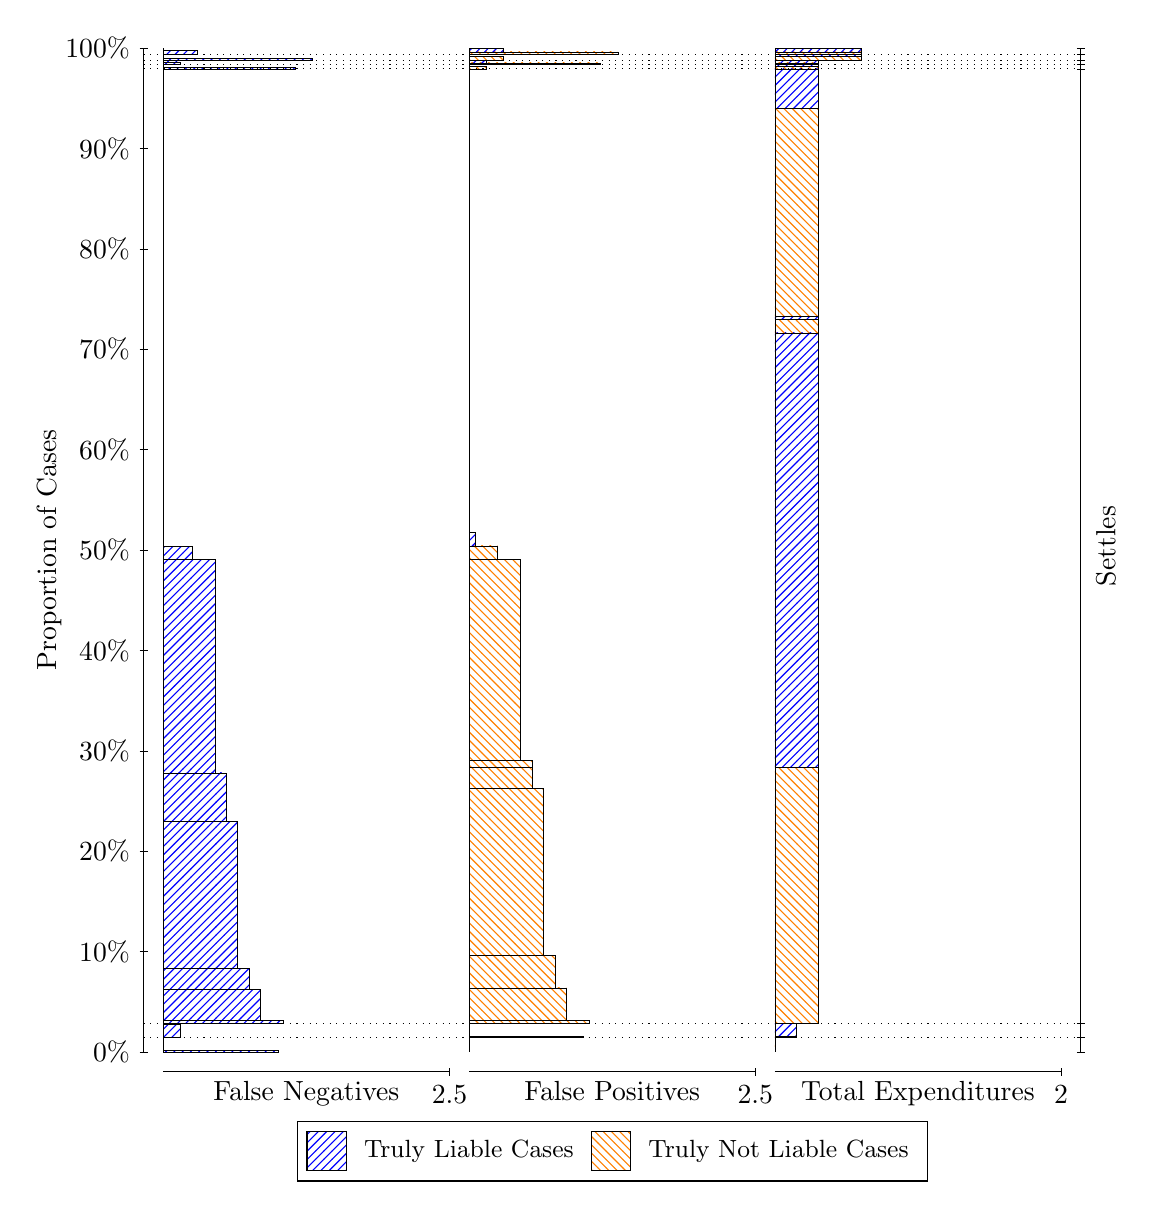
\begin{tikzpicture}
\draw[black, very thin] (1.5,1.75) -- (1.5,14.5);
\node[rotate=90, text=black, anchor=center] at (0.3, 8.125) {Proportion of Cases};
\draw[black, very thin] (1.45,1.75) -- (1.55,1.75);
\node[text=black, anchor=east] at (1.45, 1.75) {0\%};
\draw[black, very thin] (1.45,3.025) -- (1.55,3.025);
\node[text=black, anchor=east] at (1.45, 3.025) {10\%};
\draw[black, very thin] (1.45,4.3) -- (1.55,4.3);
\node[text=black, anchor=east] at (1.45, 4.3) {20\%};
\draw[black, very thin] (1.45,5.575) -- (1.55,5.575);
\node[text=black, anchor=east] at (1.45, 5.575) {30\%};
\draw[black, very thin] (1.45,6.85) -- (1.55,6.85);
\node[text=black, anchor=east] at (1.45, 6.85) {40\%};
\draw[black, very thin] (1.45,8.125) -- (1.55,8.125);
\node[text=black, anchor=east] at (1.45, 8.125) {50\%};
\draw[black, very thin] (1.45,9.4) -- (1.55,9.4);
\node[text=black, anchor=east] at (1.45, 9.4) {60\%};
\draw[black, very thin] (1.45,10.675) -- (1.55,10.675);
\node[text=black, anchor=east] at (1.45, 10.675) {70\%};
\draw[black, very thin] (1.45,11.95) -- (1.55,11.95);
\node[text=black, anchor=east] at (1.45, 11.95) {80\%};
\draw[black, very thin] (1.45,13.225) -- (1.55,13.225);
\node[text=black, anchor=east] at (1.45, 13.225) {90\%};
\draw[black, very thin] (1.45,14.5) -- (1.55,14.5);
\node[text=black, anchor=east] at (1.45, 14.5) {100\%};

\draw[black, very thin] (13.4,1.75) -- (13.4,14.5);
\draw[black, very thin] (13.35,1.75) -- (13.45,1.75);
\node[anchor=west] at (13.35, 1.75) {};
\draw[black, very thin] (13.35,1.9325) -- (13.45,1.9325);
\node[anchor=west] at (13.35, 1.9325) {};
\draw[black, very thin] (13.35,2.115) -- (13.45,2.115);
\node[anchor=west] at (13.35, 2.115) {};
\draw[black, very thin] (13.35,14.236) -- (13.45,14.236);
\node[anchor=west] at (13.35, 14.236) {};
\draw[black, very thin] (13.35,14.288) -- (13.45,14.288);
\node[anchor=west] at (13.35, 14.288) {};
\draw[black, very thin] (13.35,14.347) -- (13.45,14.347);
\node[anchor=west] at (13.35, 14.347) {};
\draw[black, very thin] (13.35,14.423) -- (13.45,14.423);
\node[anchor=west] at (13.35, 14.423) {};
\draw[black, very thin] (13.35,14.5) -- (13.45,14.5);
\node[anchor=west] at (13.35, 14.5) {};

\draw[black, very thin, pattern color=blue, pattern=north east lines] (1.75,1.75) rectangle (3.2033,1.7692);
\draw[black, very thin, pattern color=orange, pattern=north west lines] (1.75,1.7692) rectangle (1.75,1.9325);
\draw[black, very thin, pattern color=blue, pattern=north east lines] (1.75,1.9325) rectangle (1.968,2.0958);
\draw[black, very thin, pattern color=orange, pattern=north west lines] (1.75,2.0958) rectangle (1.75,2.115);
\draw[black, very thin, pattern color=blue, pattern=north east lines] (1.75,2.115) rectangle (3.276,2.1523);
\draw[black, very thin, pattern color=blue, pattern=north east lines] (1.75,2.1523) rectangle (2.9853,2.5478);
\draw[black, very thin, pattern color=blue, pattern=north east lines] (1.75,2.5478) rectangle (2.84,2.8087);
\draw[black, very thin, pattern color=blue, pattern=north east lines] (1.75,2.8087) rectangle (2.6947,4.6753);
\draw[black, very thin, pattern color=blue, pattern=north east lines] (1.75,4.6753) rectangle (2.5493,5.2958);
\draw[black, very thin, pattern color=blue, pattern=north east lines] (1.75,5.2958) rectangle (2.404,8.004);
\draw[black, very thin, pattern color=blue, pattern=north east lines] (1.75,8.004) rectangle (2.1133,8.1742);
\draw[black, very thin, pattern color=orange, pattern=north west lines] (1.75,8.1742) rectangle (1.75,14.236);
\draw[black, very thin, pattern color=blue, pattern=north east lines] (1.75,14.236) rectangle (3.4213,14.258);
\draw[black, very thin, pattern color=orange, pattern=north west lines] (1.75,14.258) rectangle (1.75,14.288);
\draw[black, very thin, pattern color=blue, pattern=north east lines] (1.75,14.288) rectangle (1.968,14.323);
\draw[black, very thin, pattern color=orange, pattern=north west lines] (1.75,14.323) rectangle (1.75,14.347);
\draw[black, very thin, pattern color=blue, pattern=north east lines] (1.75,14.347) rectangle (3.6393,14.373);
\draw[black, very thin, pattern color=orange, pattern=north west lines] (1.75,14.373) rectangle (1.75,14.423);
\draw[black, very thin, pattern color=blue, pattern=north east lines] (1.75,14.423) rectangle (2.186,14.473);
\draw[black, very thin, pattern color=orange, pattern=north west lines] (1.75,14.473) rectangle (1.75,14.5);
\draw[black, very thin, pattern color=orange, pattern=north west lines] (5.6333,1.75) rectangle (5.6333,1.9133);
\draw[black, very thin, pattern color=blue, pattern=north east lines] (5.6333,1.9133) rectangle (5.6333,1.9325);
\draw[black, very thin, pattern color=orange, pattern=north west lines] (5.6333,1.9325) rectangle (7.0867,1.9517);
\draw[black, very thin, pattern color=blue, pattern=north east lines] (5.6333,1.9517) rectangle (5.6333,2.115);
\draw[black, very thin, pattern color=orange, pattern=north west lines] (5.6333,2.115) rectangle (7.1593,2.1523);
\draw[black, very thin, pattern color=orange, pattern=north west lines] (5.6333,2.1523) rectangle (6.8687,2.5641);
\draw[black, very thin, pattern color=orange, pattern=north west lines] (5.6333,2.5641) rectangle (6.7233,2.9756);
\draw[black, very thin, pattern color=orange, pattern=north west lines] (5.6333,2.9756) rectangle (6.578,5.1012);
\draw[black, very thin, pattern color=orange, pattern=north west lines] (5.6333,5.1012) rectangle (6.4327,5.3666);
\draw[black, very thin, pattern color=orange, pattern=north west lines] (5.6333,5.3666) rectangle (6.4327,5.4563);
\draw[black, very thin, pattern color=orange, pattern=north west lines] (5.6333,5.4563) rectangle (6.2873,8.0068);
\draw[black, very thin, pattern color=orange, pattern=north west lines] (5.6333,8.0068) rectangle (5.9967,8.177);
\draw[black, very thin, pattern color=blue, pattern=north east lines] (5.6333,8.177) rectangle (5.706,8.3472);
\draw[black, very thin, pattern color=blue, pattern=north east lines] (5.6333,8.3472) rectangle (5.6333,14.236);
\draw[black, very thin, pattern color=orange, pattern=north west lines] (5.6333,14.236) rectangle (5.8513,14.266);
\draw[black, very thin, pattern color=blue, pattern=north east lines] (5.6333,14.266) rectangle (5.6333,14.288);
\draw[black, very thin, pattern color=orange, pattern=north west lines] (5.6333,14.288) rectangle (7.3047,14.312);
\draw[black, very thin, pattern color=blue, pattern=north east lines] (5.6333,14.312) rectangle (5.8513,14.347);
\draw[black, very thin, pattern color=orange, pattern=north west lines] (5.6333,14.347) rectangle (6.0693,14.397);
\draw[black, very thin, pattern color=blue, pattern=north east lines] (5.6333,14.397) rectangle (5.6333,14.423);
\draw[black, very thin, pattern color=orange, pattern=north west lines] (5.6333,14.423) rectangle (7.5227,14.45);
\draw[black, very thin, pattern color=blue, pattern=north east lines] (5.6333,14.45) rectangle (6.0693,14.5);
\draw[black, very thin, pattern color=orange, pattern=north west lines] (9.5167,1.75) rectangle (9.5167,1.9133);
\draw[black, very thin, pattern color=blue, pattern=north east lines] (9.5167,1.9133) rectangle (9.5167,1.9325);
\draw[black, very thin, pattern color=orange, pattern=north west lines] (9.5167,1.9325) rectangle (9.7892,1.9517);
\draw[black, very thin, pattern color=blue, pattern=north east lines] (9.5167,1.9517) rectangle (9.7892,2.115);
\draw[black, very thin, pattern color=orange, pattern=north west lines] (9.5167,2.115) rectangle (10.062,5.3666);
\draw[black, very thin, pattern color=blue, pattern=north east lines] (9.5167,5.3666) rectangle (10.062,10.883);
\draw[black, very thin, pattern color=orange, pattern=north west lines] (9.5167,10.883) rectangle (10.062,11.053);
\draw[black, very thin, pattern color=blue, pattern=north east lines] (9.5167,11.053) rectangle (10.062,11.09);
\draw[black, very thin, pattern color=orange, pattern=north west lines] (9.5167,11.09) rectangle (10.062,13.73);
\draw[black, very thin, pattern color=blue, pattern=north east lines] (9.5167,13.73) rectangle (10.062,14.236);
\draw[black, very thin, pattern color=orange, pattern=north west lines] (9.5167,14.236) rectangle (10.062,14.266);
\draw[black, very thin, pattern color=blue, pattern=north east lines] (9.5167,14.266) rectangle (10.062,14.288);
\draw[black, very thin, pattern color=orange, pattern=north west lines] (9.5167,14.288) rectangle (10.062,14.312);
\draw[black, very thin, pattern color=blue, pattern=north east lines] (9.5167,14.312) rectangle (10.062,14.347);
\draw[black, very thin, pattern color=orange, pattern=north west lines] (9.5167,14.347) rectangle (10.607,14.397);
\draw[black, very thin, pattern color=blue, pattern=north east lines] (9.5167,14.397) rectangle (10.607,14.423);
\draw[black, very thin, pattern color=orange, pattern=north west lines] (9.5167,14.423) rectangle (10.607,14.45);
\draw[black, very thin, pattern color=blue, pattern=north east lines] (9.5167,14.45) rectangle (10.607,14.5);
\draw[black, dotted] (1.5,1.9325) -- (13.4,1.9325);
\draw[black, dotted] (1.5,2.115) -- (13.4,2.115);
\draw[black, dotted] (1.5,14.236) -- (13.4,14.236);
\draw[black, dotted] (1.5,14.288) -- (13.4,14.288);
\draw[black, dotted] (1.5,14.347) -- (13.4,14.347);
\draw[black, dotted] (1.5,14.423) -- (13.4,14.423);
\draw[black, very thin] (1.75,1.5) -- (5.3833,1.5);
\node[text=black, anchor=north] at (3.5667, 1.5) {False Negatives};
\draw[black, very thin] (5.3833,1.45) -- (5.3833,1.55);
\node[text=black, anchor=north] at (5.3833, 1.45) {2.5};

\draw[black, very thin] (5.6333,1.5) -- (9.2667,1.5);
\node[text=black, anchor=north] at (7.45, 1.5) {False Positives};
\draw[black, very thin] (9.2667,1.45) -- (9.2667,1.55);
\node[text=black, anchor=north] at (9.2667, 1.45) {2.5};

\draw[black, very thin] (9.5167,1.5) -- (13.15,1.5);
\node[text=black, anchor=north] at (11.333, 1.5) {Total Expenditures};
\draw[black, very thin] (13.15,1.45) -- (13.15,1.55);
\node[text=black, anchor=north] at (13.15, 1.45) {2};



\node[text=black, centered, rotate=90] at (13.72, 8.1756) {Settles};





\draw (7.449999999999999,1.5) node[draw=none] (baseCoordinate) {};
\begin{scope}[align=center]
        \matrix[scale=0.5, draw=black, below=0.5cm of baseCoordinate, nodes={draw}, column sep=0.1cm]{
            \node[rectangle, draw, minimum width=0.5cm, minimum height=0.5cm, pattern color=blue, pattern=north east lines] {}; &
            \node[draw=none, font=\small, text=black] (B) {Truly Liable Cases}; &
            \node[rectangle, draw, minimum width=0.5cm, minimum height=0.5cm, pattern color=orange, pattern=north west lines] {}; &
            \node[draw=none, font=\small, text=black] (B) {Truly Not Liable Cases}; \\
            };
\end{scope}

\end{tikzpicture}
\end{document}